\section{Muhammad Abdul Gani Wijaya 1174071}
\subsection{DATA GEOSPASIAL} 
Geospasial terdiri dari dua kata, yaitu geo dan spasial. Geo berarti bumi dan spasial berarti ruang. Data geospasial adalah aspek keruangan dari suatu objek, atau yang mencakup lokasi, letak, dan posisinya. Data geospasial dipecah menjadi dua, yaitu data grafis/geometris dan data atribut/tematik. Data grafis adalah data yang terdiri dari tiga elemen yaitu titik, garis, dan luasan yang berbentuk vector maupun raster. Yang kedua adalah data atribut atau data tematik.
\begin{figure}[!htbp]
\centering
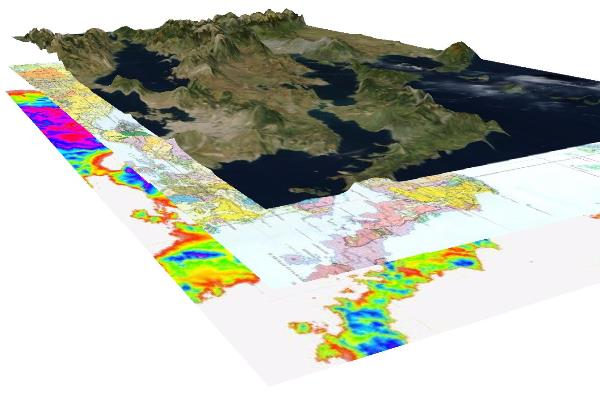
\includegraphics[width=6cm,height=6cm]{figures/Tugas1/1174071/Geospasial.jpg}
\caption{Data Geospasial}
\end{figure}	
\subsection{DATA GEOSPASIAL RASTER}
Data raster adalah data yang disimpan dalam bentuk grid atau petak sehingga terbentuk suatu ruang yang teratur dalam bentuk pixel (picture element). Foto digital seperti areal fotografi atau satelit merupakan bagian dari data raster pada peta.
\begin{figure}[!htbp]
\centering
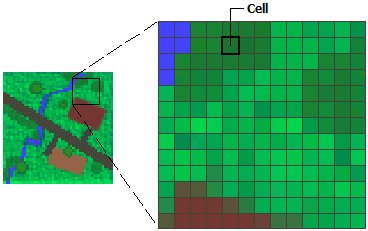
\includegraphics[width=6cm,height=6cm]{figures/Tugas1/1174071/Raster.png}
\caption{Data Raster}
\end{figure}	
\subsection{DATA GEOSPASIAL VEKTOR}
Data vector adalah data yang disimpan dalam bentuk koordinat titik yang menampilkan, menempatkan, dan menyimpan data spasial dengan menggunakan titik, garis, atau polygon. Terdapat tiga jenis data vector yaitu titik, garis, dan polygon. Tipe data ini biasanya terdapat pada peta. Setiap bagian dari data vector bias saja mempunyai informasi yang berasolasi satu sama lain.
\begin{figure}[!htbp]
\centering
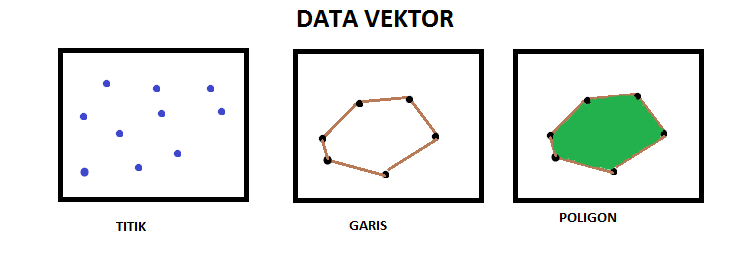
\includegraphics[width=6cm,height=6cm]{figures/Tugas1/1174071/Vektor.PNG}
\caption{Data Vektor}
\end{figure}	
\subsection {DATA GEOSPASIAL (OPEN GEOSPASIAL CONSORTIUM)}
Open Geospasial Consortium (OGC) Web Services (OWS) adalah layanan yang didefinisikan oleh OGC, yang memungkinkan semua jenis fungsi geospasial. Layanan yang ada pad OGC ini termasuk layanan untuk akses data, tampilan data dan pengolahan data. Permintaan OWS didefinisikan dengan menggunakan protocol Hyper Text Transfer Protocol (HTTP) dan dikodekan menggunakan struktur keyvaluepair (KVP) atau Exentible Markuo Language (XML). OWS yang paling banyak dikenal adalah Web Map Services (WMS).
\begin{figure}[!htbp]
\centering
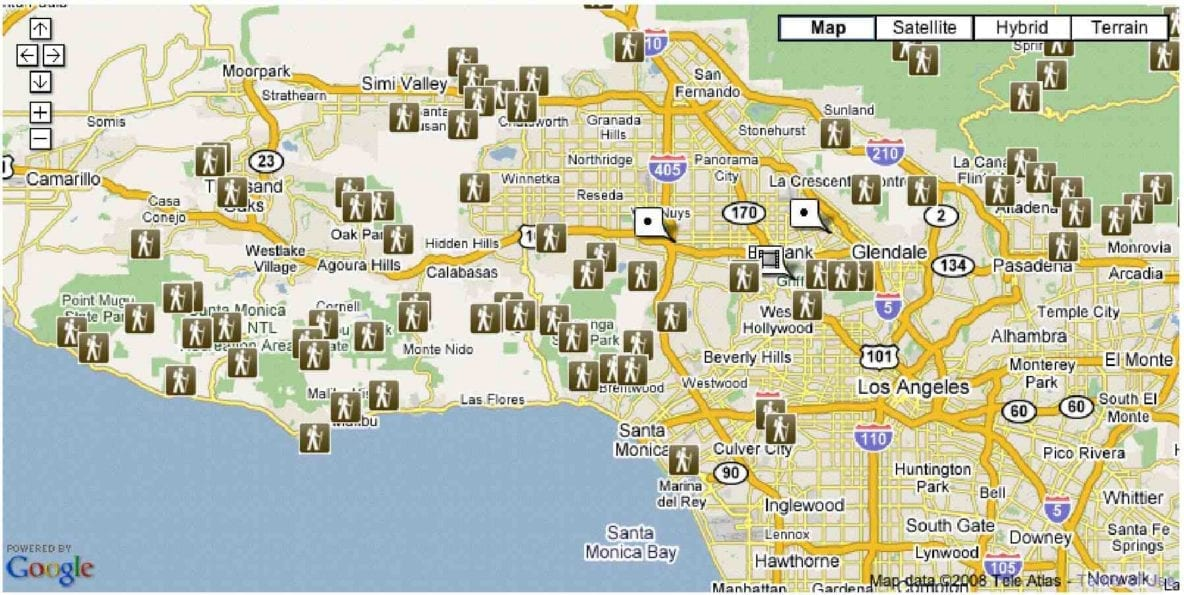
\includegraphics[width=6cm,height=6cm]{figures/Tugas1/1174071/OGC.jpg}
\caption{Open Geospasial Consortium}
\end{figure}
\subsection {Link Youtube}
https://youtu.be/unKOdRU1z4E
\subsection {Check Plagiarism}
\begin{figure}
\centering
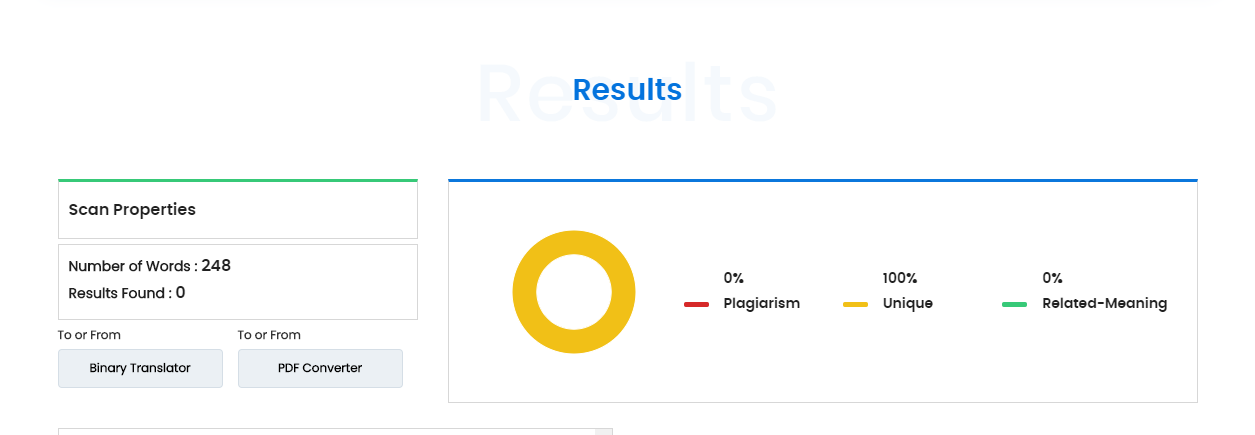
\includegraphics[width=15cm,height=10cm]{figures/Tugas1/1174071/Plagiarism.png}
\caption{Check Plagiarism}
\end{figure}